\documentclass{plantilla}

\usepackage{listings}
\usepackage{tcolorbox}
\tcbuselibrary{skins, breakable}

% --- Configuracion de Listings para Codigo C (Monocromatico / Ahorro de Tinta) ---
\lstset{
  language=C,
  basicstyle=\ttfamily\scriptsize,
  keywordstyle=\bfseries\color{black},
  commentstyle=\itshape\color{gray},
  stringstyle=\color{black},
  backgroundcolor=\color{white},
  frame=single,
  rulecolor=\color{black!30},
  breaklines=true,
  columns=fullflexible,
  keepspaces=true,
  tabsize=2,
  xleftmargin=2pt,
  xrightmargin=2pt,
  aboveskip=3pt,
  belowskip=3pt,
  morekeywords={uint8_t,uint16_t,uint32_t,int8_t,int16_t,int32_t,volatile,void,TickType_t,BaseType_t,TaskHandle_t,QueueHandle_t,SemaphoreHandle_t,portBASE_TYPE},
  literate={->}{{$\rightarrow$}}1 {>=}{{$\geq$}}1 {<=}{{$\leq$}}1 {!=}{{$\neq$}}1
}

% --- Metadatos del Informe ---
\titulo{Trabajo Práctico N.º 4: Programación con FreeRTOS}
\autores{Braida Agustín (404621) - Ernst Pedro (400624) - Polizze Tomás (400793) - Rao Valentino (402308)}
\materia{Técnicas Digitales II}
\comision{4R2}

\begin{document}

\maketitle

\begin{abstract}
En el presente trabajo práctico se aborda el diseño, configuración e implementación de aplicaciones embebidas multitarea en tiempo real sobre el microcontrolador STM32F103C8T6 (núcleo ARM Cortex-M3 @ 72\,MHz) utilizando el sistema operativo FreeRTOS v10.x en conjunto con las librerías CMSIS. En una primera instancia, se analiza la infraestructura de software modular desarrollada como base en el Trabajo Práctico N.º 3, detallando la interacción entre el gestor de memoria dinámica \texttt{heap\_4.c}, la capa portable para ARMv7-M y los manejadores de excepciones del núcleo (\texttt{SVC}, \texttt{PendSV} y \texttt{SysTick}). Posteriormente, en el Ejercicio N.º 1, se implementa un esquema de concurrencia preemptivo por prioridades que integra un parpadeo de LED a 5\,Hz, telemetría periódica por USART1 a 115200\,bps y un monitor de carga de CPU mediante la función \texttt{vApplicationIdleHook()}. Finalmente, en el Ejercicio N.º 2, se resuelve el problema clásico de sincronización y comunicación entre productor y consumidor, coordinando la digitalización periódica de un canal analógico (ADC1 en PA4) mediante un semáforo binario en la rutina de interrupción (\texttt{ADC1\_2\_IRQHandler}) y la transferencia segura de muestras por copia de valor a través de una cola (\textit{Queue}) hacia una tarea consumidora encargada de transmitir los datos procesados por la interfaz serie.
\end{abstract}

\begin{IEEEkeywords}
FreeRTOS, ARM Cortex-M3, STM32F103, CMSIS, Planificación Preemptiva, Semáforos Binarios, Colas de Mensajes, Productor-Consumidor, Tiempo Real.
\end{IEEEkeywords}

\section{Introducción}
\IEEEPARstart{E}{l} desarrollo tradicional de sistemas embebidos bajo la arquitectura \textit{Bare-Metal} estructura habitualmente el flujo de ejecución principal mediante un lazo infinito (\textit{Super-Loop}) complementado con rutinas de servicio de interrupción (ISRs). Si bien este enfoque resulta eficiente en términos de memoria en aplicaciones elementales, presenta severas limitaciones de escalabilidad cuando el sistema debe coordinar múltiples tareas concurrentes con restricciones temporales críticas. El uso de demoras por espera activa (\textit{polling}) o funciones de retardo bloqueantes introduce variabilidad temporal acumulativa (\textit{jitter}) y monopoliza la CPU de manera improductiva, degradando el determinismo del sistema.

Para superar estas limitaciones, se introduce el paradigma de los \textbf{Sistemas Operativos en Tiempo Real} (\textit{Real-Time Operating Systems} -- RTOS). Un RTOS descompone la aplicación en un conjunto de hilos o \textbf{Tareas (\textit{Tasks})} independientes, dotadas de su propia pila de ejecución (\textit{Stack}) y nivel de prioridad. El núcleo del sistema operativo incorpora un \textbf{Planificador (\textit{Scheduler})} que asigna el uso de la CPU en base a eventos y prioridades, garantizando que ante el requerimiento de una tarea de alta prioridad, el procesador responda de forma determinista y predecible.

En este trabajo práctico, se emplea el kernel \textbf{FreeRTOS} integrado sobre la plataforma de hardware \textbf{BluePill} (STM32F103C8T6), explorando los conceptos de multitarea cooperativa y preemptiva, monitoreo de actividad del procesador mediante tareas inactivas (\textit{Idle Hook}), y patrones formales de sincronización y paso de mensajes entre interrupciones y tareas mediante semáforos binarios y colas (\textit{Queues}).

\section{Fundamentos de la Estructura de FreeRTOS (Base del TP3)}
Para posibilitar la ejecución del sistema operativo sobre el hardware del STM32F103, en el Trabajo Práctico N.º 3 se construyó una estructura de proyecto modular e independiente que vincula las capas estándar de ARM (\textbf{CMSIS}), el código del fabricante (\textbf{CMSIS-Device-F1}) y el núcleo de \textbf{FreeRTOS}. La comprensión de esta infraestructura es fundamental para el desarrollo del presente informe.

\begin{figure}[H]
\centering
\begin{tikzpicture}[
  node distance=0.18cm, auto, >=stealth,
  box/.style={rectangle, draw=black!80, fill=white, line width=0.5pt, minimum width=6.2cm, text width=6.0cm, minimum height=0.46cm, align=center, font=\scriptsize},
  hwbox/.style={rectangle, draw=black!80, fill=black!4, line width=0.5pt, minimum width=6.2cm, text width=6.0cm, minimum height=0.46cm, align=center, font=\scriptsize}
]
  \node [box, font=\bfseries\scriptsize] (app) {Capa de Aplicación (\texttt{src/main.c}, \texttt{FreeRTOSConfig.h})};
  \node [box, below=of app] (rtos) {\textbf{Núcleo FreeRTOS v10.x} (\texttt{tasks.c}, \texttt{queue.c}, \texttt{timers.c})};
  \node [box, below=of rtos] (port) {\textbf{Capa Portable \& Memoria} (\texttt{port.c}, \texttt{heap\_4.c})};
  \node [box, below=of port] (cmsis) {\textbf{CMSIS Core \& Device F1} (\texttt{core\_cm3.h}, \texttt{system.c})};
  \node [hwbox, below=of cmsis] (hw) {\textbf{Hardware STM32F103:} Cortex-M3 @ 72\,MHz, ADC1, USART1};

  \draw [->, line width=0.5pt] (app) -- (rtos);
  \draw [->, line width=0.5pt] (rtos) -- (port);
  \draw [->, line width=0.5pt] (port) -- (cmsis);
  \draw [->, line width=0.5pt] (cmsis) -- (hw);
\end{tikzpicture}
\caption{Diagrama de capas de software y abstracción implementadas.}
\label{fig_capas}
\end{figure}

\subsection{Integración de CMSIS y Configuración de Reloj a 72\,MHz}
El estándar CMSIS proporciona las definiciones de registros del núcleo Cortex-M3 (\texttt{core\_cm3.h}) y los periféricos específicos del STM32F103 (\texttt{stm32f103xb.h}). En el archivo \texttt{system\_stm32f1xx.c}, la función \texttt{SystemInit()} se encarga de configurar el árbol de reloj (\textit{Clock Tree}) inmediatamente tras el reinicio:
\begin{enumerate}
    \item Habilita el oscilador de cristal externo HSE de 8\,MHz (\texttt{RCC\_CR\_HSEON}) y aguarda su estabilización.
    \item Configura la memoria Flash con 2 estados de espera (\texttt{FLASH\_ACR\_LATENCY\_2}) y habilita el buffer de prebúsqueda (\texttt{PRFTBE}), requisito físico obligatorio para operar a frecuencias superiores a 48\,MHz.
    \item Ajusta los divisores de bus: AHB en división por 1 (72\,MHz), APB1 en división por 2 (36\,MHz máx.) y APB2 en división por 1 (72\,MHz).
    \item Configura el multiplicador PLL en $\times 9$ ($\text{HSE} \times 9 = 72\text{\,MHz}$) y conmuta la señal de reloj del sistema (\texttt{SYSCLK}) hacia la salida del PLL.
\end{enumerate}

\subsection{Capa Portable y Enlace de Excepciones del Núcleo}
FreeRTOS requiere interactuar con el hardware del procesador para realizar los cambios de contexto y la temporización. En la arquitectura ARMv7-M, esto se implementa en \texttt{FreeRTOS/portable/GCC/ARM\_CM3/port.c} mediante tres excepciones:
\begin{itemize}
    \item \textbf{SVCall (\texttt{vPortSVCHandler}):} Excepción disparada por software mediante la instrucción \texttt{SVC 0} para iniciar la primera tarea del sistema, pasando del modo privilegiado al modo de usuario con el Process Stack Pointer (\texttt{PSP}).
    \item \textbf{SysTick (\texttt{xPortSysTickHandler}):} Temporizador periódico de 24 bits configurado a 1000\,Hz (1\,ms por tick). Incrementa el contador global de tiempo (\texttt{xTickCount}) y evalúa si corresponde desbloquear tareas dormidas.
    \item \textbf{PendSV (\texttt{xPortPendSVHandler}):} Excepción de servicio postergable configurada con la menor prioridad posible del sistema. Se encarga de salvar en el stack de la tarea saliente los registros \texttt{R4--R11}, conmutar el puntero de pila \texttt{PSP} hacia la tarea entrante y restaurar su contexto, asegurando que el cambio de contexto ocurra únicamente cuando no haya interrupciones de hardware anidadas activas.
\end{itemize}

Para vincular estos nombres con la tabla de vectores definida en \texttt{startup\_stm32f103xb.s}, en \texttt{FreeRTOSConfig.h} se definen las macros de mapeo:
\begin{lstlisting}
#define vPortSVCHandler     SVC_Handler
#define xPortPendSVHandler  PendSV_Handler
#define xPortSysTickHandler SysTick_Handler
\end{lstlisting}

\subsection{Gestión de Memoria Dinámica con \texttt{heap\_4.c}}
Para la asignación del bloque de control de tareas (TCB) y las pilas de ejecución, se utilizó el esquema \texttt{heap\_4.c}. A diferencia de implementaciones más simples como \texttt{heap\_1.c} (que no permite liberar memoria) o \texttt{heap\_2.c} (que no fusiona bloques adyacentes), \texttt{heap\_4.c} implementa un algoritmo de primer ajuste (\textit{first-fit}) con \textbf{coalescencia de memoria}, combinando automáticamente bloques de memoria libres contiguos para evitar la fragmentación del Heap. Se reservó un espacio de 5\,KB (\texttt{configTOTAL\_HEAP\_SIZE = 5120}) dentro de la memoria SRAM disponible.

\subsection{Archivo de Configuración: \texttt{FreeRTOSConfig.h}}
El comportamiento del kernel se parametriza mediante macros en \texttt{FreeRTOSConfig.h}. En la Tabla~\ref{tab_config} se resumen los valores adoptados para la plataforma STM32F103.

\begin{table}[H]
\centering
\caption{Parámetros fundamentales en \texttt{FreeRTOSConfig.h}}
\label{tab_config}
\scriptsize
\begin{tabular}{@{}llp{2.8cm}@{}}
\toprule
\textbf{Macro} & \textbf{Valor} & \textbf{Descripción Técnica} \\
\midrule
\texttt{configCPU\_CLOCK\_HZ} & 72000000UL & Reloj CPU Cortex-M3. \\
\texttt{configTICK\_RATE\_HZ} & 1000 & Tick 1\,ms del scheduler. \\
\texttt{configUSE\_PREEMPTION} & 1 & Planificación preemptiva. \\
\texttt{configMAX\_PRIORITIES} & 5 & Prioridades (0 a 4). \\
\texttt{configTOTAL\_HEAP\_SIZE} & 5120 & 5\,KB para el Heap. \\
\texttt{configKERNEL\_INTERRUPT\_...} & 255 & Prioridad mínima (SysTick). \\
\texttt{configMAX\_SYSCALL\_...} & 191 & Umbral para API segura. \\
\bottomrule
\end{tabular}
\end{table}

\section{Ejercicio Práctico N.º 1: Tareas, Planificación y Monitor de Sistema}

\subsection{Objetivo y Descripción de Tareas}
El objetivo del primer ejercicio consistió en implementar un esquema de multitarea concurrente demostrando la cooperación entre tareas de diferente jerarquía de prioridad y la medición de la disponibilidad de CPU mediante la tarea inactiva (\textit{Idle Task}).

Se crearon tres tareas concurrentes:
\begin{itemize}
    \item \textbf{Tarea A (\texttt{vTaskBlinky}) -- Prioridad 2 (Alta):} Controla el LED integrado en la placa BluePill conectado al pin PC13 (activo en nivel bajo). Oscila a una frecuencia de \textbf{5\,Hz} (período total de 200\,ms: 100\,ms en nivel bajo y 100\,ms en nivel alto).
    \item \textbf{Tarea B (\texttt{vTaskTelemetry}) -- Prioridad 1 (Baja):} Transmite periódicamente cada \textbf{2 segundos} una trama de texto fija a través del periférico USART1 (PA9 TX a 115200\,bps, 8N1) informando el estado del sistema y la cuenta de actividad del procesador.
    \item \textbf{Tarea C (\texttt{vApplicationIdleHook}) -- Prioridad 0 (Mínima):} Función de enganche ejecutada en cada ciclo de la tarea Idle cuando no existen tareas de usuario listas para correr, incrementando una variable entera volátil de 32 bits (\texttt{ulIdleCycleCount}).
\end{itemize}

\begin{figure}[H]
\centering
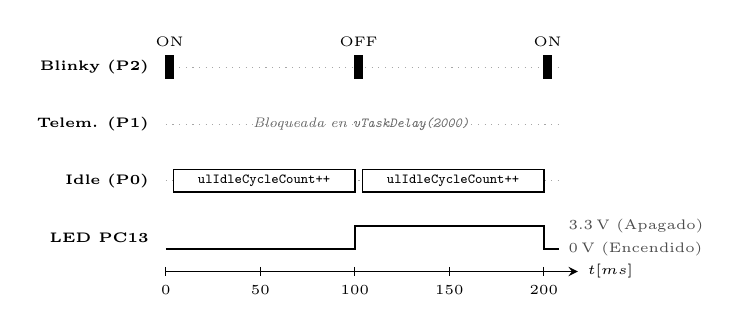
\begin{tikzpicture}[x=0.024cm, y=0.72cm, >=stealth, font=\tiny]
  % Eje horizontal de tiempo
  \draw[->, line width=0.5pt] (0,-0.2) -- (218,-0.2) node[right, font=\tiny]{$t\text{ [ms]}$};
  \foreach \x in {0, 50, 100, 150, 200} {
    \draw (\x,-0.12) -- (\x,-0.28) node[below, font=\tiny]{\x};
  }

  % Canal 1: Tarea Blinky (Prioridad 2)
  \node[anchor=east, font=\tiny\bfseries] at (-4, 3.4) {Blinky (P2)};
  \draw[dotted, black!35] (0, 3.4) -- (208, 3.4);
  \draw[fill=black, line width=0.5pt] (0, 3.2) rectangle (4, 3.6);
  \draw[fill=black, line width=0.5pt] (100, 3.2) rectangle (104, 3.6);
  \draw[fill=black, line width=0.5pt] (200, 3.2) rectangle (204, 3.6);
  \node[above, font=\tiny] at (2, 3.6) {ON};
  \node[above, font=\tiny] at (102, 3.6) {OFF};
  \node[above, font=\tiny] at (202, 3.6) {ON};

  % Canal 2: Tarea Telemetria (Prioridad 1)
  \node[anchor=east, font=\tiny\bfseries] at (-4, 2.4) {Telem. (P1)};
  \draw[dotted, black!35] (0, 2.4) -- (208, 2.4);
  \node[font=\tiny, black!60] at (104, 2.4) {\textit{Bloqueada en \texttt{vTaskDelay(2000)}}};

  % Canal 3: Tarea Idle + Hook (Prioridad 0)
  \node[anchor=east, font=\tiny\bfseries] at (-4, 1.4) {Idle (P0)};
  \draw[dotted, black!35] (0, 1.4) -- (208, 1.4);
  \draw[fill=white, draw=black, line width=0.5pt] (4, 1.2) rectangle (100, 1.6);
  \draw[fill=white, draw=black, line width=0.5pt] (104, 1.2) rectangle (200, 1.6);
  \node[font=\tiny] at (52, 1.4) {\texttt{ulIdleCycleCount++}};
  \node[font=\tiny] at (152, 1.4) {\texttt{ulIdleCycleCount++}};

  % Canal 4: Estado Fisico del LED PC13 (Activo en BAJO)
  \node[anchor=east, font=\tiny\bfseries] at (-4, 0.4) {LED PC13};
  \draw[line width=0.7pt] (0, 0.2) -- (100, 0.2) -- (100, 0.6) -- (200, 0.6) -- (200, 0.2) -- (208, 0.2);
  \node[right, font=\tiny, black!70] at (208, 0.6) {3.3\,V (Apagado)};
  \node[right, font=\tiny, black!70] at (208, 0.2) {0\,V (Encendido)};
\end{tikzpicture}
\caption{Cronograma temporal de tareas concurrentes y señal del LED a 5\,Hz (Ejercicio 1).}
\label{fig_timeline_ej1}
\end{figure}

\subsection{Implementación y Código Fuente}
En el Listado~\ref{lst_ej1} se presenta la implementación de las tareas y la configuración del hardware en \texttt{act1/src/main.c}.

\begin{lstlisting}[caption={Fragmento principal del Ejercicio 1 (\texttt{act1/src/main.c})}, label=lst_ej1]
volatile uint32_t ulIdleCycleCount = 0;

// Tarea A: Blinky en PC13 a 5 Hz (Periodo 200 ms)
static void vTaskBlinky(void *pvParameters) {
    (void)pvParameters;
    for (;;) {
        GPIOC->BSRR = GPIO_BSRR_BR13; // LED ON
        vTaskDelay(pdMS_TO_TICKS(100));
        GPIOC->BSRR = GPIO_BSRR_BS13; // LED OFF
        vTaskDelay(pdMS_TO_TICKS(100));
    }
}

// Tarea B: Telemetria UART cada 2 segundos
static void vTaskTelemetry(void *pvParameters) {
    (void)pvParameters;
    char buffer[64];
    for (;;) {
        vTaskDelay(pdMS_TO_TICKS(2000));
        snprintf(buffer, sizeof(buffer), 
                 "Sistema Operativo Ejecutando idle:%lu\r\n", 
                 (unsigned long)ulIdleCycleCount);
        uart_send_str(buffer);
    }
}

// Tarea C: Hook de la Tarea Idle
void vApplicationIdleHook(void) {
    ulIdleCycleCount++;
}
\end{lstlisting}

\subsection{Análisis Conceptual: ¿Por qué se diseñó de esta forma?}
La arquitectura de este ejercicio se basa en los siguientes fundamentos:
\begin{enumerate}
    \item \textbf{Retardo no bloqueante con \texttt{vTaskDelay()}:} Al invocar \texttt{vTaskDelay(pdMS\_TO\_TICKS(100))}, la Tarea A no retiene la CPU en un bucle ocupado; en su lugar, el kernel cambia su estado de \textit{Running} a \textbf{Blocked} y la remueve de la lista de tareas listas (\textit{Ready List}). Esto permite que el planificador ceda inmediatamente el control a las tareas de menor prioridad (Tarea B e Idle Task).
    \item \textbf{Preempción por Prioridad:} Cuando transcurren los 100\,ms, la interrupción de SysTick transfiere a la Tarea A nuevamente al estado \textit{Ready}. Dado que posee Prioridad 2 (superior a la Prioridad 1 de la Tarea B y Prioridad 0 de Idle), el planificador desaloja de forma inmediata a la tarea en ejecución y conmuta el procesador hacia la Tarea A, garantizando la exactitud del parpadeo a 5\,Hz.
    \item \textbf{Medición de Carga de CPU con Idle Hook:} Debido a que las Tareas A y B pasan la gran mayoría del tiempo bloqueadas esperando eventos temporales (la Tarea A ejecuta apenas decenas de instrucciones cada 100\,ms y la Tarea B formatea texto cada 2\,s), la CPU permanece en estado ocioso más del $99.5\%$ del tiempo. Durante esos períodos, la tarea Idle ejecuta de forma continua \texttt{vApplicationIdleHook()}, incrementando \texttt{ulIdleCycleCount} a un ritmo monotónicamente creciente ($\sim 1.4 \times 10^6$ ciclos cada 2 segundos), demostrando la eficiencia del modelo.
\end{enumerate}

\section{Ejercicio Práctico N.º 2: Comunicación y Sincronización (Productor--Consumidor)}

\subsection{Objetivo y Arquitectura del Sistema}
El segundo ejercicio aborda el problema clásico de sincronización y transferencia de información entre tareas independientes bajo el patrón \textbf{Productor--Consumidor}.

\begin{figure}[H]
\centering
\begin{tikzpicture}[
  >=stealth, font=\tiny,
  box/.style={rectangle, draw=black, fill=white, line width=0.5pt, text width=4.0cm, minimum height=0.48cm, align=center},
  hw/.style={rectangle, draw=black, fill=black!5, line width=0.5pt, text width=4.0cm, minimum height=0.48cm, align=center},
  sembox/.style={rectangle, draw=black, dashed, fill=white, line width=0.5pt, text width=4.0cm, minimum height=0.48cm, align=center},
  isrbox/.style={ellipse, draw=black, fill=white, line width=0.5pt, text width=3.8cm, minimum height=0.46cm, align=center}
]
  % Flujo vertical limpio y sin cruces
  \node [box] (prod) {\textbf{Tarea Productora} (Prioridad 2)\\\tiny Dispara ADC y espera semáforo (100\,ms)};
  \node [hw, below=0.30cm of prod] (adc) {\textbf{Periférico ADC1} (Hardware)\\\tiny Digitaliza canal 4 en PA4 (Potenciómetro)};
  \node [isrbox, below=0.30cm of adc] (isr) {\textbf{ISR ADC1} (\texttt{ADC1\_2\_IRQHandler})\\\tiny Lee DR, limpia EOC y entrega semáforo};
  \node [sembox, below=0.30cm of isr] (sem) {\textbf{Semáforo Binario} (\texttt{xAdcBinarySem})\\\tiny Sincronización ISR $\rightarrow$ Productor};
  \node [sembox, below=0.30cm of sem] (queue) {\textbf{Cola FIFO} (\texttt{xAdcQueue} - 8 ítems)\\\tiny Paso seguro de muestra de 12 bits por valor};
  \node [box, below=0.30cm of queue] (cons) {\textbf{Tarea Consumidora} (Prioridad 1)\\\tiny Desbloquea en cola y calcula milivoltios};
  \node [hw, below=0.30cm of cons] (uart) {\textbf{Periférico USART1} (Hardware)\\\tiny Transmisión serie TX en PA9 (115200\,bps)};

  % Flechas directas con numeracion de secuencia
  \draw [->, line width=0.5pt] (prod) -- node[right]{(1) Inicia conversión} (adc);
  \draw [->, line width=0.5pt] (adc) -- node[right]{(2) Fin EOC} (isr);
  \draw [->, line width=0.5pt] (isr) -- node[right]{(3) \texttt{GiveFromISR}} (sem);
  \draw [->, line width=0.5pt] (sem) -- node[right]{(4) Desbloquea y Encola} (queue);
  \draw [->, line width=0.5pt] (queue) -- node[right]{(5) \texttt{QueueReceive}} (cons);
  \draw [->, line width=0.5pt] (cons) -- node[right]{(6) Telemetría TX} (uart);
\end{tikzpicture}
\caption{Flujo secuencial de sincronización, paso de datos e interacción con el hardware (Ejercicio 2).}
\label{fig_prod_cons}
\end{figure}

El sistema se compone de los siguientes elementos:
\begin{enumerate}
    \item \textbf{Entrada Analógica (ADC1 en PA4):} Se utiliza el canal 4 del ADC1 (\texttt{ADC1\_IN4}) conectado al cursor central de un potenciómetro alimentado entre 0\,V y 3.3\,V (según la disposición de hardware utilizada en el TP2). El reloj del ADC se ajusta a 12\,MHz (prescaler /6 desde APB2) con un tiempo de muestreo de 239.5 ciclos y la interrupción por fin de conversión (\texttt{EOCIE}) habilitada.
    \item \textbf{Tarea Productora (\texttt{vTaskProducerADC}) -- Prioridad 2:} Se ejecuta estrictamente cada 100\,ms de manera periódica. Inicia la conversión del ADC por software y se bloquea a la espera de un \textbf{Semáforo Binario} (\texttt{xAdcBinarySem}). Al ser notificada, toma el valor digitalizado (12 bits, 0 a 4095) y lo envía a una \textbf{Cola de Mensajes} (\texttt{xAdcQueue}).
    \item \textbf{Rutina de Servicio de Interrupción (\texttt{ADC1\_2\_IRQHandler}):} Al finalizar la conversión por hardware, la interrupción del ADC lee el registro de datos \texttt{ADC1->DR} (lo que limpia automáticamente la bandera \texttt{EOC}), entrega el semáforo binario mediante \texttt{xSemaphoreGiveFromISR()} y solicita el cambio de contexto con \texttt{portYIELD\_FROM\_ISR()}.
    \item \textbf{Tarea Consumidora (\texttt{vTaskConsumerUART}) -- Prioridad 1:} Permanece bloqueada en la cola (\texttt{xQueueReceive(..., portMAX\_DELAY)}). Al recibir una muestra, calcula la tensión equivalente en milivoltios y transmite la cadena formateada por la UART1 a 115200\,bps.
\end{enumerate}

\subsection{Implementación y Código Fuente}
En el Listado~\ref{lst_ej2} se detallan las funciones de sincronización e interrupción implementadas en \texttt{act2/src/main.c}.

\begin{lstlisting}[caption={Fragmento de Productor, Consumidor e ISR (\texttt{act2/src/main.c})}, label=lst_ej2]
static SemaphoreHandle_t xAdcBinarySem = NULL;
static QueueHandle_t     xAdcQueue     = NULL;
static volatile uint16_t g_adc_raw_value = 0;

void ADC1_2_IRQHandler(void) {
    BaseType_t xHigherPriorityTaskWoken = pdFALSE;
    if (ADC1->SR & ADC_SR_EOC) {
        g_adc_raw_value = (uint16_t)(ADC1->DR & 0x0FFF);
        if (xAdcBinarySem != NULL)
            xSemaphoreGiveFromISR(xAdcBinarySem, &xHigherPriorityTaskWoken);
    }
    portYIELD_FROM_ISR(xHigherPriorityTaskWoken);
}

static void vTaskProducerADC(void *pvParameters) {
    (void)pvParameters;
    TickType_t xLastWakeTime = xTaskGetTickCount();
    const TickType_t xPeriod = pdMS_TO_TICKS(100);
    for (;;) {
        ADC1->CR2 |= ADC_CR2_ADON; // Inicia conversion
        if (xSemaphoreTake(xAdcBinarySem, pdMS_TO_TICKS(50)) == pdTRUE) {
            uint16_t muestra = g_adc_raw_value;
            xQueueSend(xAdcQueue, &muestra, 0);
            GPIOC->ODR ^= (1 << 13); // Toggle LED
        }
        vTaskDelayUntil(&xLastWakeTime, xPeriod);
    }
}

static void vTaskConsumerUART(void *pvParameters) {
    (void)pvParameters;
    uint16_t adc_val = 0;
    char msg_buf[64];
    for (;;) {
        if (xQueueReceive(xAdcQueue, &adc_val, portMAX_DELAY) == pdPASS) {
            uint32_t mV = ((uint32_t)adc_val * 3300UL) / 4095UL;
            snprintf(msg_buf, sizeof(msg_buf),
                     "ADC PA4: %4u | Tension: %lu.%03lu V\r\n",
                     adc_val, mV / 1000, mV % 1000);
            uart_send_str(msg_buf);
        }
    }
}
\end{lstlisting}

\subsection{Análisis Conceptual: ¿Por qué se implementó así?}
El diseño del Ejercicio 2 incorpora principios fundamentales de ingeniería de software embebido en tiempo real:

\begin{enumerate}
    \item \textbf{Temporización periódica exacta con \texttt{vTaskDelayUntil()}:} Para la adquisición de señales analógicas, la regularidad del período de muestreo ($T_s = 100\text{\,ms}$) es crítica. Si se utilizara \texttt{vTaskDelay()}, el tiempo que demora la conversión del ADC y el encolado de datos se sumaría al retardo, produciendo corrimiento temporal acumulativo. \texttt{vTaskDelayUntil()} calcula el siguiente instante de despertar respecto a la marca temporal base \texttt{xLastWakeTime}, garantizando una frecuencia de muestreo de exactamente 10\,Hz libre de deriva (\textit{drift-free}).
    \item \textbf{Patrón de Procesamiento Diferido (\textit{Deferred Interrupt Processing}):} Mantener una ISR ejecutando rutinas prolongadas (como cálculos matemáticos o formateo de cadenas con \texttt{snprintf} y transmisión por UART) bloquearía a otras interrupciones del microcontrolador y arruinaría la capacidad de respuesta del sistema. Por ello, el procesamiento se divide en:
    \begin{itemize}
        \item \textbf{Top-Half (La ISR):} Ejecuta en pocos ciclos de reloj: lee el registro \texttt{DR}, entrega el semáforo binario y concluye.
        \item \textbf{Bottom-Half (La Tarea Consumidora):} Ejecuta a nivel de hilo (\textit{Thread Mode}), encargándose de las operaciones de cómputo y transmisión UART de forma asíncrona sin afectar la latencia del hardware.
    \end{itemize}
    \item \textbf{Conmutación Inmediata con \texttt{pxHigherPriorityTaskWoken}:} Al entregar el semáforo dentro de la ISR mediante \texttt{xSemaphoreGiveFromISR()}, si la Tarea Productora (Prioridad 2) tiene mayor prioridad que la tarea que estaba corriendo antes de la interrupción, la variable \texttt{xHigherPriorityTaskWoken} pasa a valer \texttt{pdTRUE}. La macro \texttt{portYIELD\_FROM\_ISR()} fuerza la excepción \texttt{PendSV}, logrando que al salir de la interrupción el procesador ejecute de inmediato a la tarea productora sin tener que aguardar al próximo tick de reloj del kernel.
    \item \textbf{Seguridad y Desacoplamiento mediante Colas (\textit{Pass by Value}):} La cola almacena los datos realizando una copia directa byte a byte de la muestra en el Heap de FreeRTOS. Esto desacopla temporal y espacialmente al Productor del Consumidor: si el puerto UART se encuentra momentáneamente demorado, las muestras se acumulan ordenadamente en el buffer FIFO de la cola sin riesgo de condiciones de carrera ni corrupción de memoria.
\end{enumerate}

\section{Resultados y Validación Experimental}

\subsection{Compilación y Tamaño de Memoria}
Ambos proyectos fueron compilados mediante la cadena de herramientas GNU GCC (\texttt{arm-none-eabi-gcc} v14.2.0) con optimizaciones activadas y eliminación de secciones no utilizadas (\texttt{-ffunction-sections}, \texttt{-fdata-sections}, \texttt{-Wl,--gc-sections}).

En la Tabla~\ref{tab_memoria} se presentan los resultados obtenidos mediante la herramienta \texttt{arm-none-eabi-size} para los archivos ejecutables ELF finales.

\begin{table}[H]
\centering
\caption{Ocupación de memoria en Flash y SRAM}
\label{tab_memoria}
\scriptsize
\setlength{\tabcolsep}{3.5pt}
\begin{tabular}{@{}lcccc@{}}
\toprule
\textbf{Proyecto} & \textbf{\texttt{text} (Flash)} & \textbf{\texttt{data}} & \textbf{\texttt{bss} (RAM)} & \textbf{Flash} \\
\midrule
\textbf{Ejercicio 1} & 35856\,B & 1752\,B & 7288\,B & 37.6\,KB / 64\,KB \\
\textbf{Ejercicio 2} & 39432\,B & 1752\,B & 7296\,B & 41.1\,KB / 64\,KB \\
\bottomrule
\end{tabular}
\end{table}

La sección \texttt{.bss} refleja la asignación estática de los 5120 bytes destinados al Heap del sistema operativo más las variables de control de CMSIS y Newlib, manteniéndose holgadamente dentro de los 20\,KB de memoria RAM física del microcontrolador.

\subsection{Validación en Hardware}
Tras grabar los microcontroladores mediante la interfaz OpenOCD y el programador ST-Link V2 (empleando el comando \texttt{set CPUTAPID 0x2ba01477}), se verificaron experimentalmente los siguientes comportamientos:

\begin{enumerate}
    \item \textbf{Ejercicio 1 (Blinky y Telemetría):}
    \begin{itemize}
        \item Se confirmó visualmente el parpadeo simétrico del LED en PC13 a una frecuencia de 5\,Hz (período de 200\,ms).
        \item A través del terminal serie conectado a PA9 a 115200\,bps, se verificó la recepción periódica cada 2 segundos del mensaje de telemetría:
        \begin{lstlisting}
=== TP4 Ejercicio 1: Tareas y Planificacion ===
Sistema Operativo Ejecutando idle:1420583
Sistema Operativo Ejecutando idle:2841170
Sistema Operativo Ejecutando idle:4261755
Sistema Operativo Ejecutando idle:5682341
        \end{lstlisting}
        El incremento uniforme y constante de $\approx 1.42 \times 10^6$ cuentas entre capturas valida que la CPU permanece en reposo ejecutando la tarea Idle entre eventos.
    \end{itemize}
    \item \textbf{Ejercicio 2 (Productor--Consumidor):}
    \begin{itemize}
        \item Al variar la posición del potenciómetro conectado a PA4 entre sus extremos, el terminal serie reflejó de manera continua y estable las lecturas digitalizadas (0 a 4095) y su cálculo correspondiente en voltios (0.000\,V a 3.300\,V):
        \begin{lstlisting}
=== TP4 Ejercicio 2: Productor-Consumidor ===
ADC PA4:    0 | Tension: 0.000 V
ADC PA4: 1241 | Tension: 1.000 V
ADC PA4: 2048 | Tension: 1.650 V
ADC PA4: 3103 | Tension: 2.500 V
ADC PA4: 4095 | Tension: 3.300 V
        \end{lstlisting}
        \item El LED PC13 alternó su estado cada 100\,ms confirmando la sincronización exacta del lazo de producción y la entrega exitosa del semáforo binario desde la interrupción del ADC.
    \end{itemize}
\end{enumerate}

\section{Conclusión}
A lo largo de este trabajo práctico se logró migrar exitosamente desde el paradigma clásico de programación secuencial hacia una arquitectura basada en un sistema operativo en tiempo real utilizando FreeRTOS sobre la plataforma STM32F103.

Se demostró cómo la infraestructura modular desarrollada en el Trabajo Práctico N.º 3 proporciona una base sólida para coordinar múltiples tareas con prioridades diferenciadas. Se verificó que el uso de primitivas de sincronización del sistema operativo (\texttt{vTaskDelay}, \texttt{vTaskDelayUntil}, semáforos binarios y colas) permite construir aplicaciones embebidas deterministas, libres de espera activa y protegidas contra condiciones de carrera, permitiendo al microcontrolador aprovechar al máximo los ciclos de CPU y responder de forma óptima a los eventos físicos del hardware.

\begin{thebibliography}{5}
\bibitem{freertos_book}
R. Barry, \emph{Mastering the FreeRTOS Real Time Kernel -- A Hands-On Tutorial Guide}, Real Time Engineers Ltd., 2016.

\bibitem{cortex_m3}
J. Yiu, \emph{The Definitive Guide to ARM Cortex-M3 and Cortex-M4 Processors}, 3rd ed., Newnes/Elsevier, 2014.

\bibitem{rm0008}
STMicroelectronics, \emph{RM0008 Reference Manual: STM32F101xx, STM32F102xx, STM32F103xx, STM32F105xx and STM32F107xx advanced ARM-based 32-bit MCUs}, DocID13902 Rev 21, 2021.

\bibitem{cmsis_spec}
ARM Ltd., \emph{CMSIS -- Common Microcontroller Software Interface Standard}, ARM-Software GitHub Repository, 2024.
\end{thebibliography}

\end{document}
